% reset to default value for the next chapters (because intro messed it up)
\fancyhead[LE]{\textbf{\thepage}~~~\textit{\leftmark}}
\fancyhead[RE]{\MakeUppercase{\chaptername}~\thechapter}
\fancyhead[LO]{\textit{\rightmark}}
\fancyhead[RO]{\textbf{\thepage}}

\section{Introduction}
  \label{ch01:sec:introduction}
  A language is a concept allowing one to express some meaning and communicate.
  For this thesis, we will consider languages that can be expressed by means
  of a text. A text can be viewed as a simple entity: a sequence of letters,
  numbers or symbols. But to work with texts and being able to create algorithms
  that can process them, we need to define some terms and notions. Let us define
  what are the main components of a text. The first unit that can be found in a
  text is defined by the notion of \textit{words}.

  \theoremstyle{definition}
  \begin{definition}[A word]
    \label{ch01:def:def-word}
    Let $\Sigma$ be a a finite alphabet representing a non-empty finite set of
    symbols. A word is a finite sequence of symbols from $\Sigma$ that carries a
    meaning.
  \end{definition}

  In this thesis, we are only interested in texts of occidental languages like
  English. Any further mention to \textit{a word} will refer to a sequence of
  letters (from the Roman alphabet), digits or symbols (like punctuation marks
  such as dash ``-'') that carries a meaning. Then, we can assemble words to
  form \textit{sentences}.

  \theoremstyle{definition}
  \begin{definition}[A sentence]
    \label{ch01:def:def-sentence}
    A sentence is a sequence of words, separated by spaces or punctuation
    symbols.  The first word of a sentence starts with an uppercase letter and
    the last word of the sentence is followed by a period (.), a question mark
    (?) or an exclamation mark (!).
  \end{definition}

  Sentences can be then be assembled to form \textit{a text}.

  \theoremstyle{definition}
  \begin{definition}[A text]
    \label{ch01:def:def-text}
    A text is a sequence of sentences.
  \end{definition}

  Another important notion when working with text is the \textit{vocabulary}.

  \theoremstyle{definition}
  \begin{definition}[A vocabulary]
    \label{ch01:def:def-vocabulary}
    The vocabulary of a text is the set of all the unique words which occur in
    this text.
  \end{definition}

  The length of a text should not be confused with the size of its vocabulary.
  Indeed, if a word appears several times in a text, it will be present only
  once in its vocabulary. Therefore, the length of a text is usually way larger
  than the size of its vocabulary. Let us take an example of two short texts to
  illustrate this.~\autoref{ch01:tab:vocabulary-text-example} indicates the
  vocabulary of two short texts.

  \begin{itemize}
    \item Text 1 has a vocabulary size of 17 words but a text length of 23
      words.
    \item Text 2 has a vocabulary size of 17 words but a text length of 20
      words.
  \end{itemize}

  \begin{table}[t]
    \resizebox{\textwidth}{!}{
    \centering
    \begin{tabular}{llcl}
      \toprule[0.15em]
        & Text && Vocabulary\\
      \midrule[0.08em]
      1 & Add the milk to the flour and egg preparation
       && Add, the, milk, to, flour, and, \\

        & and mix it. Do not mix too quickly to avoid
       && egg, preparation, mix, it, Do, not,\\

        & lumps in the preparation.
       && too, quickly, avoid, lumps, in\\
      \midrule

      2 & Liverpool won the final against Tottenham.
       && Liverpool, won, the, final, against, \\

        & Salah scored after 1 minute and Origi scored
       && Tottenham, Salah, scored, after, 1,\\

        & another goal at the 87th minute.
       && minute, and, Origi, another, goal,\\

        &
       && at, 87th\\
      \bottomrule[0.15em]
    \end{tabular}}
    \caption{Examples of short texts and their vocabularies.}
    \label{ch01:tab:vocabulary-text-example}
  \end{table}

  \noindent When we want to talk about the length of a text, we usually use the
  term ``token'' over the term ``word''. For example, we can say that Text 1
  contains 23 tokens (because its text length is 23 words).\medskip

  In the Natural Language Processing (NLP) domain, the final objective is
  usually to solve a given task. This includes for instance text classification
  which consists in finding the correct category of a text. Another task is
  information retrieval which focuses on extracting the correct sentences or
  documents the most relevant to a question. In order to show how the vocabulary
  of a text can be used to solve a given task, let us pick up the example of the
  text classification task. In this task, a naive way to find the correct
  category of a text would be to look at its tokens or at the content of its
  vocabulary and assign the category with the greatest amount of specific words
  (\textit{e.g.} the words ``won'', ``scored'' and ``goal'' of Text 2
  in~\autoref{ch01:tab:vocabulary-text-example} probably indicate that the text
  is about \textit{sport}). However, it is difficult to compare two texts based
  solely on their vocabulary. Some words are different but have the same
  meaning, so two texts can have completely different vocabularies but still
  discuss the same subject or have the same information. The same goes for
  information retrieval, as a sentence can be the perfect answer to a question
  without using any of the words of the question. Therefore, although tokens and
  vocabularies are the essence of texts, there are not sufficient to represent
  the semantic information of the text or to process the content of the
  document. In order to solve this issue, we need additional concepts or
  representations that can be used to work with texts or documents. The next
  section presents some notions that are commonly used in the NLP literature.

\section{From words to numerical representations}
  In the vocabulary of a text, each word only appears once even if it has
  several occurrences in the text. Therefore the vocabulary representation of a
  text is lacking some information, which is a shortcoming to be able to process
  it. If one text contains 20 times the word ``football'' and another text
  contains it only once, there is no way to know which text speaks the most
  about \textit{football} by only looking at their vocabulary because both text
  vocabularies have only a single occurrence of ``football''. One solution to
  this problem is the \textit{Bag-of-Words (BoW)}
  representation~\citep{lang1995newsweeder, joachims1997probabilistic}.

  \theoremstyle{definition}
  \begin{definition}[Bag-of-Words]
    \label{ch01:def:def-bow}
    The Bag-of-Words representation of a text is the set of all the unique words
    within it, and the associated number of occurrence of each word.
  \end{definition}

  \noindent For the two texts of~\autoref{ch01:tab:vocabulary-text-example},
  their Bag-of-Words are:

  \begin{itemize}
    \item Text 1: \\
      \{
      Add:~1,
      the:~3,
      milk:~1,
      to:~2,
      flour:~1,
      and:~2,
      egg:~1,
      preparation:~2,
      mix:~2,
      it:~1,
      Do:~1,
      not:~1,
      too:~1,
      quickly:~1,
      avoid:~1,
      lumps:~1,
      in:~1
      \}
    \item Text 2:\\
      \{
      Liverpool:~1,
      won:~1,
      the:~2,
      final:~1,
      against:~1,
      Tottenham:~1,
      Salah:~1,
      scored:~2,
      after:~1,
      1:~1,
      minute:~2,
      and:~1,
      Origi:~1,
      another:~1,
      goal:~1,
      at:~1,
      87th:~1
      \}
  \end{itemize}

  With Bag-of-Words representations, one can tell if among two texts using the
  same words, one contains more terms related to a subject. But solving this
  problem also introduces another one. In a text, most of the words are
  irrelevant to understand its topic. For example, in Text 2, the words
  ``another'' or ``after'' are less important than ``scored'' or ``goal'' to
  know that the text deals about \textit{football}. Moreover, if a word appears
  in a lot of texts, then it is probably not discriminative to know the topic of
  a text. For instance, the word ``minute'' in Text 2 can also be found in other
  cooking recipes (which is the topic of Text 1) so this word is not indicative
  to differentiate the two different topics. To take into account the fact that
  less important words are usually way more frequent than more specific ones (it
  has been shown empirically that the frequency of words in a text follows a
  Zipf's law) and therefore that the number of occurrences of a word is not an
  indicative information, the values in BoW need to be replaced. The values need
  to measure the importance of a term in a text, but also among a set of texts.
  Words that are frequent among all the texts should have a smaller value
  because they are not discriminative. On the other hand, less frequent words
  should have a higher value because they better characterize a text. One
  solution is to replace the number of occurrences by the \textit{TF-IDF value}.

  \theoremstyle{definition}
  \begin{definition}[TF-IDF]
    The TF-IDF of a word is a statistical value that indicates the importance of
    a word within a text among a collection of texts. It is defined as:
    \begin{equation}
      \text{TF-IDF}(word, text) = tf_{word, text} \times
      \log(\frac{N}{D_{word}})
    \end{equation}
    \label{ch01:def:def-tfidf}
  \end{definition}

  \noindent where $tf_{word, text}$ is the number of occurrences of $word$ in
  $text$, $N$ is the total number of texts and $D_{word}$ is the number of texts
  which contain $word$. With the same texts as
  in~\autoref{ch01:tab:vocabulary-text-example}, we have:

  \begin{itemize}
    \item TF-IDF(``the'', Text 1) = $3 \times \log (\frac{2}{2})$ = 0
    \item TF-IDF(``the'', Text 2) = $2 \times \log (\frac{2}{2})$ = 0
    \item TF-IDF(``milk'', Text 1) = $1 \times \log (\frac{2}{1})$ = 0.693
    \item TF-IDF(``scored'', Text 2) = $2 \times \log (\frac{2}{1})$ = 1.39
  \end{itemize}

  \medskip
  Now that we have introduced the concept of TF-IDF, we can have a
  representation for each document based on the words it contains and the
  importance of each word. This type of representation has been proved to be
  useful for information retrieval~\citep{ramos2003using} or document
  classification~\citep{zhang2011comparative}. However, this representation has
  some severe limitations:

  \begin{enumerate}
    \item In order to compute the similarity of two given texts or to find the
      most specific words in a BoW representation, one has to go through each
      element and compare the words or their value. This becomes a problem when
      the size of the vocabulary is in the order of thousands and the number of
      texts reach several millions.
    \item These representations can be viewed as \textit{manually} generated.
      While the process of finding the unique words and counting their number of
      occurrences can be automated, the definition used to compute the weights
      (\textit{i.e.} the values) in the BoW representations are defined by a
      human, which implies the need of an expert who knows what values would be
      useful for processing texts.
    \item The BoW representation has zero understanding of the semantic and
      syntactic properties of words. Indeed, with the BoW representation, there
      is no way to know that ``car'' and ``vehicle'' are related words, unless a
      human annotator has explicitely indicated it (which brings us to point
      2.).
  \end{enumerate}

  To overcome these limitations, a solution is to find another way to represent
  texts, sentences and words. Moreover, with the increasing power of computers
  and the development of new models, these representations should have some
  properties to perform computations on them. Therefore, this brings \textbf{the
  need a numerical representation of the language}, which is \textbf{capable of
  encoding the linguistic information} inside it.

\section{Word vectors}
  In classic Machine Learning (this notion will be defined in more details in
  \autoref{chap:ml-for-we}), a standard approach consists in encoding
  information as numerical vectors. A vector can be viewed as an array of
  numerical values. For example, if a person is 33 years old, has 2 cars and
  lives in a 1000 square feet house, then it can be represented by the vector:
  $[33, 2, 1000]$. The values in the vectors are the characteristics of this
  person. Following this idea, NLP scientists have proposed to represent words
  of a language also as arrays of values. This notion of arrays of values comes
  from a mathematical background, so let us first define some concepts we will
  use throughout this thesis.

  \theoremstyle{definition}
  \begin{definition}[A vector space, simplified version]
    \label{ch01:def:def-vector-space}
    A vector space $\mathcal{X}$ over $\mathbb{R}$ is a collection of vectors
    and a set of two operations with specific properties which can be used on
    vectors:
    \begin{enumerate}
      \item vector addition: adding two vectors $\mathbf{u}, \mathbf{v} \in
        \mathcal{X}$ produces another vector which is also in $\mathcal{X}$.
      \item scalar multiplication: multiplying a vector $\mathbf{u} \in
        \mathcal{X}$ with a scalar $\lambda \in \mathbb{R}$ produces another
        vector which also belongs to $\mathcal{X}$.
    \end{enumerate}
  \end{definition}

  A \textit{vector space} is a generic concept and it can be composed
  of different kind of objects like matrices or functions (but all the elements
  of a vector space must be of the same nature). For the rest of this thesis, we
  will consider vector spaces which are either $\mathbb{R}^d$ or a subspace of
  it. Another important notion is the concept of \textit{vectors} and more
  precisely \textit{d-dimensional} vectors.

  \theoremstyle{definition}
  \begin{definition}[A vector]
    \label{ch01:def:def-vector}
    A vector is an element of a vector space $\mathcal{X}$. In this thesis, we
    will consider vectors of $\mathbb{R}^d$ (or vectors from $\mathcal{X}
    \subseteq \mathbb{R}^d$). In this case, we say that $\mathbf{v} \in
    \mathbb{R}^d$ is a \textit{d-dimensional} vector because it is composed of a
    sequence of \textit{d} values, each one belonging to $\mathbb{R}$. From a
    practical point of view, we will write the values of a
    \textit{d-dimensional} vector as $[\mathbf{v}_{[1]},~\mathbf{v}_{[2]},~...,
    ~\mathbf{v}_{[d]}]$.
  \end{definition}

  In classic Machine Learning, vectors are used as numerical representations of
  data. In the small example above, the vector $[33, 2, 1000] \in \mathbb{R}^3$
  is the numerical representation of the person. In natural language processing,
  the problem is to find a numerical representation of the language which
  encodes linguistic information. As we have seen in
  \autoref{ch01:sec:introduction}, the smallest units of meaning in a text are
  words, so first we need to find a numerical representation for each word of a
  vocabulary. A naive way to find such representations is to associate a
  \textit{one-hot vector} to each word.
  In~\autoref{ch01:tab:onehot-vectors-example}, we have associated a one-hot
  vector to each word of a simplified vocabulary (which comes
  from~\autoref{ch01:tab:vocabulary-text-example}). In one-hot vectors, all
  values are 0 except for one value which is equal to 1. The length of one-hot
  vectors is the same as the size of the vocabulary, which allows to associate a
  vector different from the others to each word by placing the 1 at a position
  which is specific to each word.\medbreak

  \begin{table}[htb]
    \centering
    \begin{tabular}{llcl}
      \toprule[0.15em]
        & Word && One-hot vector\\
      \midrule[0.08em]
      1  & Add         && \{1, 0, 0, 0, 0, 0, 0, 0, 0, 0\}\\
      2  & the         && \{0, 1, 0, 0, 0, 0, 0, 0, 0, 0\}\\
      3  & milk        && \{0, 0, 1, 0, 0, 0, 0, 0, 0, 0\}\\
      4  & to          && \{0, 0, 0, 1, 0, 0, 0, 0, 0, 0\}\\
      5  & flour       && \{0, 0, 0, 0, 1, 0, 0, 0, 0, 0\}\\
      6  & and         && \{0, 0, 0, 0, 0, 1, 0, 0, 0, 0\}\\
      7  & egg         && \{0, 0, 0, 0, 0, 0, 1, 0, 0, 0\}\\
      8  & preparation && \{0, 0, 0, 0, 0, 0, 0, 1, 0, 0\}\\
      9  & mix         && \{0, 0, 0, 0, 0, 0, 0, 0, 1, 0\}\\
      10 & it          && \{0, 0, 0, 0, 0, 0, 0, 0, 0, 1\}\\
      \bottomrule[0.15em]
    \end{tabular}
    \caption[Examples of one-hot vectors associated to each word of a small
    vocabulary.]{Examples of one-hot vectors associated to each word of a small
    vocabulary (10 words). Vectors have 10 dimensions because the vocabulary is
    composed of 10 words.}
    \label{ch01:tab:onehot-vectors-example}
  \end{table}

  \noindent More formally, one-hot vectors are defined as follows.

  \theoremstyle{definition}
  \begin{definition}[A one-hot vector]
    \label{ch01:def:def-onehot}
    A one-hot vector of \textit{d} dimensions is an element \textbf{v} of the
    vector space $\mathbb{B}^d \subseteq \mathbb{R}^d$ where $\mathbb{B} = \{0,
    1\}$ and:
    \begin{equation}
      \sum_{i=1}^d \mathbf{v}_{[i]} = 1
    \end{equation}
  \end{definition}

  As said before, the dimension $d$ is set to be equal to the size of the
  vocabulary. In the rest of this thesis, we will write \textbf{onehot(k)} to
  identify the one-hot vector where the $k$-th value is the one equal to $1$.
  Then we can associate a unique vector to each one of the words of the
  vocabulary based on their position in this vocabulary. For example, in
  \autoref{ch01:tab:onehot-vectors-example}, the word ``preparation'' is at the
  8-th position in the vocabulary, so it is associated with the vector
  $\mathbf{onehot(8)} = \{0, 0, 0, 0, 0, 0, 0, 1, 0, 0\}$. Each word will
  therefore have a different vector, because $\mathbf{onehot(i)} \neq
  \mathbf{onehot(j)} \text{ if } i \neq j$.\medskip

  BoW representations have some limitations, one of them being that it is not
  straightforward to compute the similarity of two different texts with their
  BoW representations. Indeed, words in BoW of two texts are not necessarily the
  same so one has to compare words one by one to know what are the common ones.
  When the words or sentences of a document or the document itself are
  represented with elements of a vector space, like one-hot vectors which are
  elements of a boolean vector space, the mathematical properties of vector
  spaces allow one to use vector operations and similarity functions defined
  over the vector spaces. The mathematical properties of vector spaces solve
  some issues raised by the BoW representations, mainly the computation of the
  distance between two representations to compare them (which can be calculated
  with a function defined over the vector space like the Euclidean distance for
  $\mathbb{R}^d$). Moreover, one-hot vectors also solve the BoW representations
  issue of handcrafted vector values like with TF-IDF because values in one-hot
  vectors are independent of the properties of the words like its number of
  occurrences in texts. However, one-hot vectors do not solve the problem of
  encoding linguistic information. Indeed, there is no way to tell if two words
  are related or not by looking at their one-hot vector representations, because
  the position of the value 1 does not depend on the properties of words but
  on their position in the vocabulary, which is not representative of their
  linguistic properties. Furthermore, the length of one-hot vectors can also
  become a problem as their length should be the same as the size of the
  vocabulary, which can be in the order of millions.

  A better numerical representation of words than one-hot vectors is to
  associate each word with a vector of real values, \textit{i.e.} associating it
  with a vector $\mathbf{v} \in \mathbb{R}^d$. This introduces the notion of
  \textit{word embeddings}.

  \theoremstyle{definition}
  \begin{definition}[Word embeddings]
    \label{ch01:def:def-word-embedding}
    The embedding of a word \textit{w} is a vector $\mathbf{v}_w \in
    \mathbb{R}^d$ where $d$ is the dimension of the embedding. The embedding
    matrix $\mathbf{M} \in \mathbb{R}^{|\mathcal{V}| \times d}$ (where
    $|\mathcal{V}|$ is the size of the vocabulary $\mathcal{V}$) is a matrix
    composed of the stacked up embeddings of all the words of the vocabulary.
  \end{definition}

  This real-valued numerical representation addresses the first two of the three
  issues of BoW representations: (i) a representation that can be used to
  compute vector operations like similarity and distances calculations; (ii) it
  does not need handcrafted expressions to be defined. However, for the last of
  the three issues (encoding linguistic information), we need to add more
  constraints. Indeed, if the values of the embeddings are chosen randomly for
  each word, then there is no way to tell if two words are related or not
  because the distance between their vectors would also be random. Therefore the
  values in the embeddings have to be carefully designed to reflect the
  linguistic properties of words.\medskip

  As an example, a common practice in the NLP literature
  \citep{mikolov2013efficient, pennington2014glove} is to set the values of the
  vectors so that words that are related or have similar meanings also have
  similar word embeddings. In~\autoref{ch01:subfig:values-embeddings-2D}, word
  embeddings of 2 dimensions (\textit{i.e.} vectors of 2 values) are reported
  for six words of the vocabularies from Text 1 and Text 2
  of~\autoref{ch01:tab:vocabulary-text-example}. The embeddings are plotted on a
  2D plan in~\autoref{ch01:subfig:plan-embeddings-2D} with the respective word
  they represent. The words ``flour'' and ``milk'' do not have the same meaning
  but they belong to the same semantic field (cooking ingredients) so their
  values are similar. The word ``lumps'' also have similar values because it is
  related to the word ``flour''. However, the words ``Liverpool'' and
  ``Tottenham'' are far from the words ``flour'' and ``milk'' on the 2D plan and
  their vector values are also quite different because they are not related to
  the semantic field of cooking and food. The word ``goal'' is closer to the two
  cities (Euclidean distance between the vectors of ``goal'' and ``Liverpool''
  is $0.447$; distance between the vectors of ``goal'' and ``flour'' is $2.332$)
  because it is more related to the football teams of the two cities than to
  some cooking ingredients.\medskip

  \begin{figure}[b!]
    \centering
    \begin{subfigure}[b]{0.38\textwidth}
      \centering
      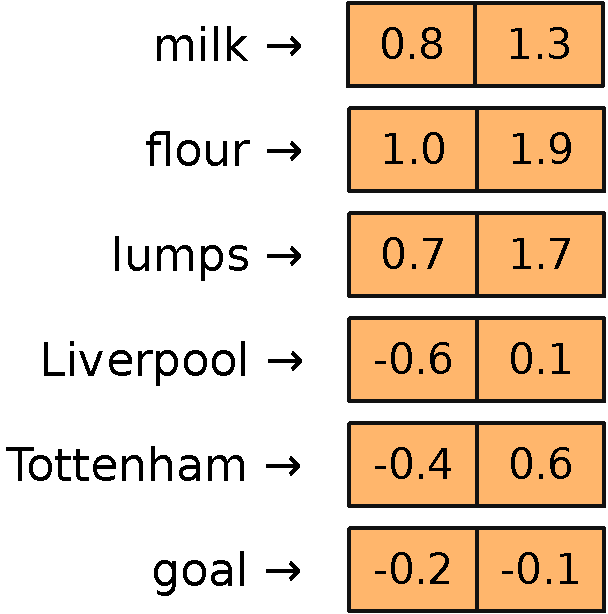
\includegraphics[width=\textwidth]{ch01-embeddings2D-vectors}
      \caption{Values of 2-dimensional word embeddings of some words.}
      \label{ch01:subfig:values-embeddings-2D}
    \end{subfigure} \hfill
    \begin{subfigure}[b]{0.58\textwidth}
      \centering
      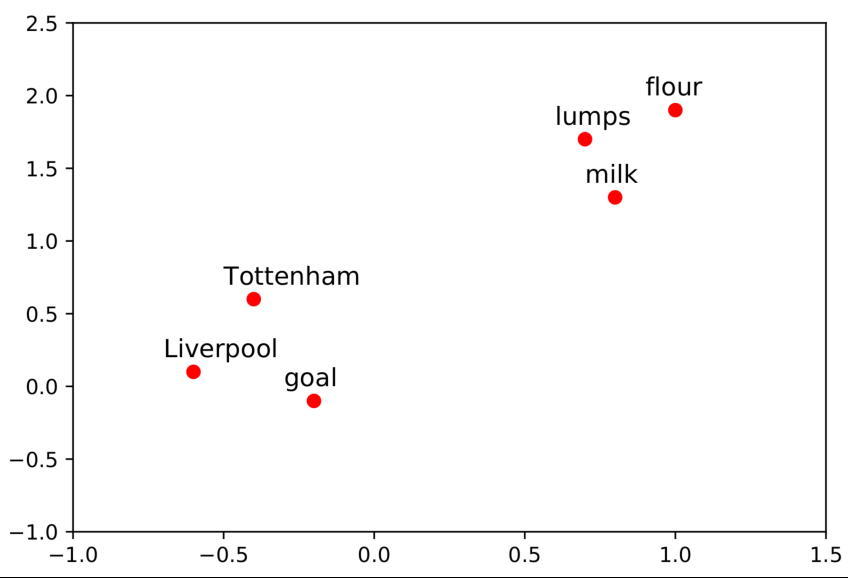
\includegraphics[width=0.98\textwidth]{ch01-embeddings2D-plan}
      \caption{Visual representation on a 2D plan of the word embeddings of some
      words.}
      \label{ch01:subfig:plan-embeddings-2D}
    \end{subfigure}
    \caption[Values and visual representations of 2-dimensional word
    embeddings.] {Values (on left subfigure) and visual representations (on
    right subfigure) of 2-dimensional word embeddings of 6 words. Values of the
    vectors have been chosen so that words that are related have similar values
    and thus are close in the 2D plan representation.}
    \label{ch01:fig:word-embeddings-2D}
  \end{figure}

  In this section, we have introduced basic ways to encode words with numerical
  representations which are commonly used in NLP models. However, there exist
  others ways to encode words like with word-cluster
  representations~\citep{bekkerman2003distributional} or using n-grams feature
  vectors~\citep{cavnar1995using}. We have seen that word embeddings have the
  ability to encode linguistic information, which is a crucial lack of one-hot
  vector representations. Other types of representations for texts (like
  sentence or document representations) can be computed either by concatenating
  or by averaging the embeddings of the words that compose it. The vector space
  $\mathbb{R}^d$ to which the word embeddings belong have some mathematical
  properties that allow one to perform vector operations like summing or
  computing the distance between two vectors. However, the vector space
  $\mathbb{R}^d$ does not have a finite size and the number of possible values
  for each word embeddings is infinite. This raises another question: among
  several word embedding representations, how to compare them and select the
  most appropriate one for our final goal, that is to solve a NLP task?

\section{Evaluation of word embeddings}
  \label{ch01:sec:word-embeddings-evaluation}
  The final objective in NLP is to solve tasks such as text classification,
  machine translation or information retrieval. Learning word embeddings is not
  a part of this final objective but rather an intermediate step to obtain
  semantic-preserving word representations that can be leveraged to solve
  downstream NLP tasks. Indeed, if the representations are able to better
  capture linguistic information into word embeddings, then downstream NLP
  models which use them to solve tasks have access to more knowledge to make
  predictions, which increases the performances on tasks~\citep{kim2016intent,
  bojanowski2016enriching}. Word embeddings can either be evaluated when they
  are created or when they are used into other models, which separates the
  evaluations into two different categories:

  \begin{enumerate}
    \item How much linguistic information is encoded into word embeddings? This
      evaluation depends only on the values in the embeddings, not on their use
      in downstream NLP tasks. We call it the \textbf{intrinsic evaluation}.
    \item How helpful are word embeddings when they are used to solve an NLP
      task? We call this the \textbf{extrinsic evaluation}.
  \end{enumerate}

  \noindent While these two types of evaluation are related, the performances of
  word embeddings on one of them do not reflect the performances on the other
  one.~\citeauthor{chiu2016intrinsic}~\citep{chiu2016intrinsic} showed that
  scores on datasets used for intrinsic evaluation are, for the majority,
  negatively correlated with scores on tasks of extrinsic evaluation which means
  that both types of evaluation are needed to evaluate word embeddings. In this
  section, we present the most common tasks and datasets used for intrinsic
  evaluation in~\autoref{ch01:subsec:intrinsic-evaluation} and for extrinsic
  evaluation in~\autoref{ch01:subsec:extrinsic-evaluation}. Most of these tasks
  require to compute the similarity or the distance between pairs of vectors, so
  let us first define in~\autoref{ch01:subsec:similarity-distance-functions}
  what are the main similarity or distance functions used in the literature.

  \subsection{Similarity and distance functions for vectors}
    \label{ch01:subsec:similarity-distance-functions}

    \subsubsection{Cosine similarity}
      Cosine similarity is computed on real-valued vectors from $\mathbb{R}^d$.
      It is the most commonly used similarity function in NLP models, and is
      also the most used one in the context of this thesis.

      \theoremstyle{definition}
      \begin{definition}[Cosine similarity]
        \label{ch01:def:def-cosine}
        The cosine similarity between two $d$-dimensional vectors $\mathbf{u},
        \mathbf{v} \in \mathbb{R}^d$ is defined as:
        \begin{equation}
          \text{cosine} (\mathbf{u}, \mathbf{v}) =
          \frac{\mathbf{u} \cdot \mathbf{v}}
          {\left\lVert \mathbf{u} \right\rVert
           \left\lVert \mathbf{v} \right\rVert} =
          \frac{\sum\limits_{i = 1}^d \mathbf{u}_{[i]} \times \mathbf{v}_{[i]}}
           {\sqrt{\sum\limits_{i = 1}^d \mathbf{u}_{[i]}^2} \times
            \sqrt{\sum\limits_{i = 1}^d \mathbf{v}_{[i]}^2}}
        \end{equation}
      \end{definition}

    \subsubsection{Jaccard similarity and Jaccard distance}
      Jaccard similarity is computed on binary vectors from $\mathbb{B}^d$ and
      has a value between 0 and 1.\\

      \theoremstyle{definition}
      \begin{definition}[Jaccard similarity]
        \label{ch01:def:def-jaccard}
        The Jaccard similarity between two binary $d$-dimensional vectors
        $\mathbf{u}, \mathbf{v} \in \mathbb{B}^d$ is defined as:
        \begin{equation}
          \text{Jaccard}_{sim} (\mathbf{u}, \mathbf{v}) =
          \frac{M_{11}}{M_{01} + M_{10} + M_{11}}
        \end{equation}
        where $M_{11}$ is the number of dimensions simultaneously set to $1$ in
        $\mathbf{u}$ and $\mathbf{v}$ and $M_{01}$ (resp. $M_{10}$) is the
        number of dimensions set to $0$ (resp. $1$) in $\mathbf{u}$ and set to
        $1$ (resp. $0$) in $\mathbf{v}$.

        \noindent Jaccard distance is closely related and is defined as:
        \begin{equation}
          \text{Jaccard}_{dist} (\mathbf{u}, \mathbf{v}) = 1 -
          \text{Jaccard}_{sim} (\mathbf{u}, \mathbf{v})
        \end{equation}
      \end{definition}

    \subsubsection{Euclidean distance}
      Euclidean distance is not a similarity function but a distance function.
      It measures how close (or how far) two vectors are.

      \theoremstyle{definition}
      \begin{definition}[Euclidean distance]
        \label{ch01:def:def-euclidean}
        The Euclidean distance between two $d$-dimensional vectors
        $\mathbf{u}, \mathbf{v} \in \mathbb{R}^d$ is defined as:
        \begin{equation}
          \text{Euclidean}_{dist} (\mathbf{u}, \mathbf{v}) =
          \sqrt{\sum\limits_{i = 1}^d (\mathbf{u}_{[i]} - \mathbf{v}_{[i]})^2}
        \end{equation}
      \end{definition}

    \subsubsection{$\text{L}_1$ distance}
      $\text{L}_1$ distance is also a distance function like the Euclidean
      distance. It can be applied to real-valued or binary vectors. However,
      this function is not differentiable which makes it hard to use in NLP
      models.

      \theoremstyle{definition}
      \begin{definition}[$\text{L}_1$ distance]
        \label{ch01:def:def-L1-distance}
        $\text{L}_1$ distance between two $d$-dimensional vectors either
        $\mathbf{u}, \mathbf{v} \in \mathbb{R}^d$ or $\mathbf{u}, \mathbf{v} \in
        \mathbb{B}^d$ is defined as:
        \begin{equation}
          \text{L}_{1} (\mathbf{u}, \mathbf{v}) = \sqrt{\sum\limits_{i = 1}^d
          \lvert \mathbf{u}_{[i]} - \mathbf{v}_{[i]} \rvert}
        \end{equation}
      \end{definition}

  \subsection{Intrinsic evaluation}
    \label{ch01:subsec:intrinsic-evaluation}
    With the defined similarity and distance functions described in the previous
    subsection, word embeddings can be evaluated in intrinsic evaluation tasks
    to measure how much linguistic information is encoded into the vectors. The
    two main existing intrinsic evaluation tasks are word semantic similarity
    and word analogy.

    \subsubsection{Word semantic similarity}
      \label{ch01:subsubsec:semantic-similarity}
      As explained in the previous section, word embeddings should encode
      linguistic information. Words with similar meaning should have close
      vector representations. The word semantic similarity task evaluates how
      well the embeddings reflect the semantic similarity of words. It is based
      on datasets composed of pairs of words. Many datasets exist, the most
      commonly used ones being WordSim-353~\citep{finkelstein2001placing} and
      Rare Words (RW)~\citep{luong2013better}. A more extensive list of
      available datasets will be presented in the contributions of this thesis
      (\autoref{chap:dict2vec} and \autoref{chap:nlb}) where they are used to
      evaluate the word embeddings learned by the models proposed in the
      contributions. For each pair of words of the datasets, a few human
      annotators have been asked to rate the similarity between the words on a
      scale of 0 to 10. Scores from all the annotators are validated with an
      inter-annotator agreement threshold and are then averaged for each pair.
      In \autoref{ch01:tab:human-scores}, some examples of such pairs and scores
      are reported.

      \begin{table}[h!]
        \centering
        \begin{tabular}{cc}
          \toprule[0.15em]
          Pairs of words & Human score\\
          \midrule
          Maradona -- football & 8.62 \\
          month -- hotel & 1.81\\
          problem -- airport & 2.38 \\
          money -- cash & 9.15\\
          \bottomrule[0.15em]
        \end{tabular}
        \caption[Examples of pairs of words and their human similarity
        scores.]{Examples of pairs of words and their similarity scores rated by
        human annotators on a scale of 0 to 10, from the WordSim-353
        dataset~\citep{finkelstein2001placing}.}
        \label{ch01:tab:human-scores}
      \end{table}

      \begin{table}[h!]
        \centering
        \begin{subtable}[h]{0.7\textwidth}
          \centering
          \begin{tabular}{lclrrr}
            \toprule[0.15em]
            Word       && \multicolumn{4}{c}{Embedding}\\
            \midrule
            Maradona   && [0.73, & 0.55, & 0.12, & 0.33]\\
            football   && [0.62, & 0.42, & 0.07, & 0.79]\\
            month      && [0.01, & -0.22,& 0.76, & -0.94]\\
            hotel      && [0.25, & 0.62, & 0.37, & 0.23]\\
            problem    && [-0.87,& -0.83,&-0.97, & 0.89]\\
            airport    && [0.22, & -0.18,& -0.19,& -0.08]\\
            money      && [-0.09,& 0.85, & 0.20, & 0.35]\\
            cash       && [0.74, & 0.72, & -0.30,& 0.26]\\
            \bottomrule[0.15em]
          \end{tabular}
          \caption{Examples of vector values associated to some words of the
          WordSim-353 dataset~\citep{finkelstein2001placing}.}
          \vspace*{1em} % to add vertical space between subtables
          \label{ch01:tab:embeddings-values}
        \end{subtable}
        \begin{subtable}[h]{0.7\textwidth}
          \centering
          \begin{tabular}{ccc}
            \toprule[0.15em]
            Pairs of words       & Human score & Cosine similarity\\
            \midrule
            Maradona -- football & 8.62        &  0.892\\
            month -- hotel       & 1.81        & -0.070\\
            problem -- airport   & 2.38        &  0.114\\
            money -- cash        & 9.15        &  0.551\\
            \bottomrule[0.15em]
          \end{tabular}
          \caption{Examples of pairs of words and their cosine similarity scores
          computed with the cosine similarity between their respective
          embeddings.}
          \label{ch01:tab:cosine-scores}
        \end{subtable}
        \caption[Vector values and cosine similarity scores of pairs of words of
        WordSim-353.] {Cosine similarity scores
        (\autoref{ch01:tab:cosine-scores}) computed with the vector values
        (\autoref{ch01:tab:embeddings-values}) of the respective embedding of
        the words of each pair.}
      \end{table}

      \pagebreak % force it to be on next page (otherwise only 2 lines on a page
      \noindent The ideal situation would be when the similarity score between
      the respective embeddings of the words of a pair (like
      ``money''--``cash'') has the exact same value as its human score.
      However, this is very unlikely to happen for all the pairs of a dataset
      (there are typically more than 100 pairs in those datasets). Therefore, we
      need to evaluate how ``close'' word embeddings are from the human
      judgement. For each pair of words, the cosine similarity between their
      respective word embeddings is computed with the values of the vectors
      (reported in~\autoref{ch01:tab:embeddings-values}). This adds a new
      column in the table of scores
      (see~\autoref{ch01:tab:cosine-scores}).\medskip

      Comparing the similarity scores of pairs of vectors to the values assigned
      by human annotators is not a good solution mainly because the similarity
      scores are usually small (between -$1$ and $1$ for the cosine similarity
      function) whereas the values of human annotations can be much larger (up
      to $10$ in the WordSim-353 dataset). Instead of directly comparing the
      vector similarities and the human scores, a better solution is to evaluate
      if the order of values is preserved. Indeed, if a pair has a high score
      assigned by annotators and a high score obtained by computing the cosine
      similarity of the vectors, then the embeddings are reflecting the human
      judgement (the words are strongly related). To evaluate if the order is
      preserved, the common method is to use the Spearman's rank correlation
      coefficient~\citep{spearman1904proof}. It measures the correlation between
      the ranks of two lists of values. It is defined as:

      \begin{equation}
        \label{ch01:eq:spearman-coefficient}
        \rho = 1 - \frac{6 \times \sum_{i = 1}^n d_i^2}
                                    {n \times (n^2 - 1)}
      \end{equation}
      where $n$ is the number of values in the two lists and $d_i$ are the
      differences of ranks in the two lists for each value. The Spearman's rank
      correlation coefficient is a real value in the [-1, 1] range. A coefficient of 1
      (resp. -1) indicates that the values of the two lists are ranked in the
      same order (resp. in reverse order). \medskip

      \noindent Let us illustrate the computation of this coefficient with an
      example. \autoref{ch01:tab:ranks-differences} is almost the same
      as~\autoref{ch01:tab:cosine-scores} except it has three new columns:

      \begin{itemize}
        \item Rank${}_{Human}$ is the rank each value of ``Human score'' would
          have if the list was sorted in decreasing order: $9.15$ is the highest
          value of the column ``Human score'' so its rank is $1$; $8.62$ is the
          second highest value so its rank is $2$, etc.
        \item Rank${}_{Cosine}$ is the rank each value of ``Cosine similarity''
          would have if the list was sorted in decreasing order: $0.892$ is the
          highest value of the column ``Cosine similarity'' so its rank is $1$;
          $0.551$ is the second highest value so its rank is $2$, etc.
        \item Rank difference ($d_i$) is the difference of Rank${}_{Human}$ and
          Rank${}_{Cosine}$ for each value.
      \end{itemize}

      \begin{table}[h!]
        \resizebox{\textwidth}{!}{
        \centering
        \begin{tabular}{cccccc}
          \toprule[0.15em]
          Pairs of words       & Human score & Rank${}_{Human}$
                         & Cosine similarity & Rank${}_{Cosine}$
                         & Rank difference ($d_i$)\\
          \midrule
          Maradona -- football & 8.62 & 2 &  0.892 & 1 & 2 - 1 = 1\\
          month -- hotel       & 1.81 & 4 & -0.070 & 4 & 4 - 4 = 0\\
          problem -- airport   & 2.38 & 3 &  0.114 & 3 & 3 - 3 = 0\\
          money -- cash        & 9.15 & 1 &  0.551 & 2 & 1 - 2 = -1\\
          \bottomrule[0.15em]
        \end{tabular}}
        \caption{Rank differences used to compute the Spearman's rank
        correlation coefficient.}
        \label{ch01:tab:ranks-differences}
      \end{table}

      \noindent Given the formula of the Spearman's rank correlation coefficient
      (\autoref{ch01:eq:spearman-coefficient}), we have:

      \begin{equation*}
        \rho = 1 - \frac{6 \times (1^2 + 0^2 + 0^2 + (\text{-}1)^2)}
                        {4 \times (4^2 - 1)}
             = 1 - \frac{6 \times (1 + 1)}{4 \times (16 - 1)}
             = 1 - \frac{12}{60} = 1 - 0.2 = 0.8
      \end{equation*}

      A Spearman's rank correlation coefficient close to 1 indicates that the
      embeddings are close to the human semantic knowledge because pairs of
      words evaluated as highly related by humans are also highly related with
      the cosine similarity of their embeddings values. Similarly, pairs of
      words rated as not related by humans also have word embeddings values
      reflecting that they are not related (low values for their cosine
      similarity). The Spearman's coefficient for this small example is $0.8$,
      which indicates that the word embeddings values are pretty good to encode
      semantic (dis)similarity of words.

    \subsubsection{Word analogy}
      \label{ch01:subsubsec:word-analogy}
      In a language, some relations or notions between words can be common. For
      example, the words ``Berlin'' and ``Germany'' can be linked by the
      relation \textit{capital of}. The same goes for the words ``Budapest'' and
      ``Hungary'' and many others. In 2013,
      \citeauthor{mikolov2013efficient}~\citep{mikolov2013efficient} analyzed
      some word embeddings and saw that they are capable of encoding such
      relations with vector operations. Relations between words such as
      \textit{capital of} can also be encoded as vectors, and adding it
      to the embedding of a capital city can produce the embedding of the
      related country. In~\autoref{ch01:fig:word-analogy}, the black arrows
      represent the \textit{analogy}, \textit{i.e.} the vector one needs to add
      to a capital city to obtain the embedding of the related country. These
      vectors are almost identical for the three examples, which suggests that
      word embeddings are able to encode the relation between a country and its
      capital city.

      \begin{figure}[h!]
        \centering
        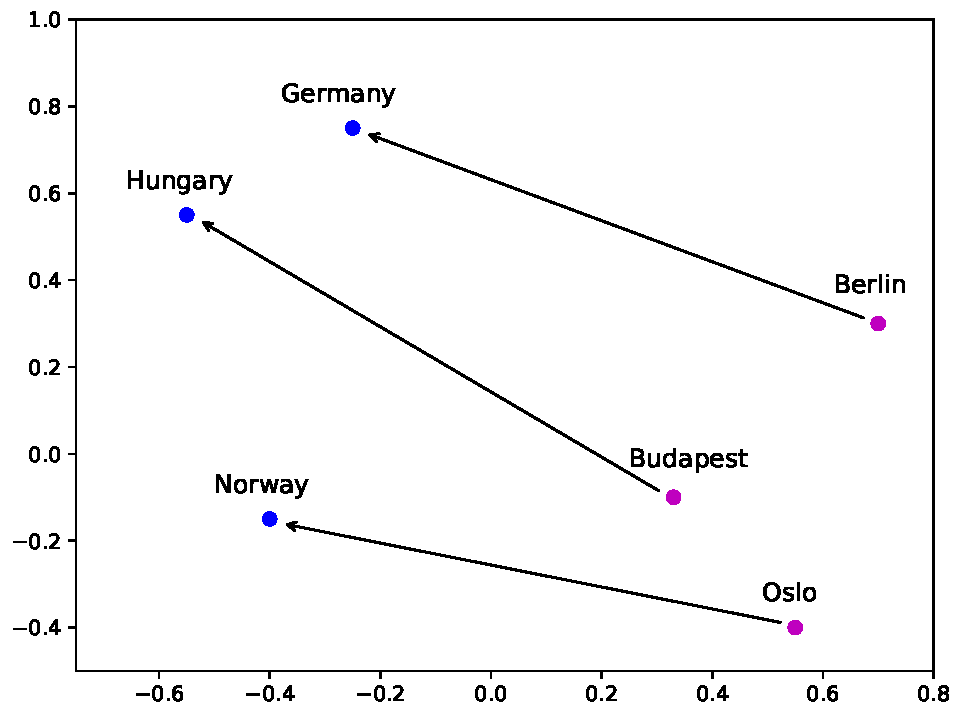
\includegraphics[width=0.85\textwidth]{ch01-word-analogy}
        \caption{Representation on a 2D plan of word embeddings and the
        analogy \textit{capital of}.}
        \label{ch01:fig:word-analogy}
      \end{figure}

      \citeauthor{mikolov2013efficient} introduced a new task to evaluate how
      well word embeddings can predict linguistic relations like ``\textit{a} is
      to \textit{b} as \textit{c} is to \textit{d}''. Their
      datasets~\citep{mikolov2013efficient} are composed of lines containing
      four words, such as ``Berlin Germany Budapest Hungary''. The task consists
      in computing the vector $\mathbf{v} = \mathbf{v}_{Germany} -
      \mathbf{v}_{Berlin} + \mathbf{v}_{Budapest}$ and see if its closest vector
      is the embedding of the word ``Hungary''. If so, the analogy is said to be
      correct. The final evaluation score for this task is the percentage of
      correctly predicted analogies. Analogies are separated into two groups:
      one focuses on semantic analogies and the other one on syntactic
      analogies, which are respectively split into 5 and 9 categories.
      \autoref{ch01:tab:word-analogy-examples} reports the different categories
      and an example for each one of them.

      \begin{table}[h]
        \resizebox{\textwidth}{!}{
        \centering
        \begin{tabular}{lccccccc}
          \toprule[0.12em]
                & & Category & & \multicolumn{4}{c}{Example (a b c d)}\\
          \midrule[0.08em]
          \textit{Semantic} & &          & & & & & \\
          && capital-common-countries && Berlin & Germany & Budapest & Hungary\\
          && capital-world && Tehran & Iran & Islamabad & Pakistan\\
          && currency && Europe & euro & Japan & yen\\
          && city-in-state && Phoenix & Arizona & Honolulu & Hawaii\\
          && family                   && king   & queen   & man      & woman\\
          \midrule
          \textit{Syntactic} & &          & & & & & \\
          && adjective-to-adverb && calm & calmly & swift & swiftly\\
          && opposite && informed & uninformed & known & unknown\\
          && comparative && cold & colder & large & larger\\
          && superlative && cold & coldest & long & longest\\
          && present-participle && debug & debugging & read & reading\\
          && nationality-adjective && Colombia & Colombian & Malta & Maltese\\
          && past-tense && flying & flew & going & went\\
          && plural && snake & snakes & pineapple & pineapples\\
          && plural-verbs && think & thinks & swim & swims\\
          \bottomrule[0.12em]
        \end{tabular}}
        \caption[Categories and examples of semantic and syntactic word
        analogies.]{Categories and examples of semantic and syntactic word
        analogies taken from the datasets of~\citep{mikolov2013efficient}.}
        \label{ch01:tab:word-analogy-examples}
      \end{table}

  \subsection{Extrinsic evaluation}
    \label{ch01:subsec:extrinsic-evaluation}
    The two intrinsic evaluations (word semantic similarity and word analogy
    tasks) described in~\autoref{ch01:subsec:intrinsic-evaluation} measure how
    well the linguistic information is encoded into word embeddings. But word
    embeddings are usually learned for another purpose, which is to be used as a
    language representation to solve a NLP task. After being learned, word
    embeddings are then fed as the input of other mathematical models that
    perform computations with them to produce representations for sentences or
    texts, and then achieve a specific goal like predicting the category of a
    text or translating a sentence. As the performance of the model to solve the
    task is dependent on the amount and the quality of linguistic information
    encoded into the word embeddings, it can be used to compare different word
    embeddings (word embeddings with more encoded information gives better
    results on the downstream tasks). The variety of tasks using word embeddings
    is large, like name entity recognition~\citep{turian2010word,
    pennington2014glove}, question answering~\citep{bordes2014open} or machine
    translation~\citep{zou2013bilingual, lample2018word}. Presenting an
    exhaustive list of all the possible tasks would be too long so we mainly
    focus on describing tasks related to document classification, which are the
    tasks used in the evaluation of the word embedding learned in the
    contributions of this thesis (see \autoref{chap:dict2vec}
    and~\autoref{chap:nlb}).

    \subsubsection{Text classification}
      \label{ch01:subsubsec:text-classification-task}
      This task aims to assign the category of a text. The text can come from
      different sources (a Wikipedia page, a newspaper, a blog article etc.)
      and the category can be of different forms (a class like ``economy'' or
      ``politics'' for a newspaper article, a hierarchical category like
      ``musician'' or ``vertebrate animal'' for a Wikipedia page, etc.). For this
      task, a model combines the embeddings of the words from the text to
      predict the correct category. The model is usually a neural network
      (neural networks will be described in~\autoref{ch02:subsec:neural-network}
      of~\autoref{chap:ml-for-we}). After the model has learned how to predict the
      correct category given a certain amount of examples (composed of texts and
      their associated category), it is evaluated on a set of texts not seen
      during the learning phase. The percentage of correctly predicted
      categories gives the score of the word embeddings for this task.

    \subsubsection{Sentiment analysis}
      This task is very similar to the text classification task. In this task,
      the objective is to predict a value given an input text, most often a
      short text like a couple of sentences. We find in this task different
      examples like predicting the number of stars (between 1 and 5) a customer
      has given to a product based on the written review of the product (
      multi-class classification tasks) or predicting if a comment about a
      service is good or bad (positive and negative \textit{i.e.} binary
      classification tasks). Like with the text classification task, another
      mathematical model is fed with word embeddings and then learns how to
      predict the correct value based on the input text. The final score for
      this task is the percentage of correctly predicted values on a set of
      unseen texts.

    \subsubsection{GLUE/SuperGLUE}
      Word embeddings are used in downstream models to solve NLP tasks. But as
      the recent downstream models become more and more
      complex~\citep{peters2018elmo, devlin2019bert}, they are able to process
      and understand more complex relations between words and sentences. Tasks
      like document classifications or sentiment analysis are not sufficient to
      evaluate the performances of the representations of words learned by these
      complex models (because their scores on those tasks reach the human
      baseline).~\citeauthor{wang2018glue}~\citep{wang2018glue} have created
      \texttt{GLUE} (\textbf{G}eneral \textbf{L}anguage \textbf{U}nderstanding
      \textbf{E}valuation benchmark), a resource of datasets to evaluate the
      performances of models on 9 downstream tasks.  \texttt{GLUE} also proposes
      tools to standardize the evaluation of models and a
      leaderboard\footnote{\url{https://gluebenchmark.com/leaderboard}} to
      compare the models proposed by different people. The nine tasks in
      \texttt{GLUE} are:

      \begin{itemize}
        \item \texttt{CoLA}: a set of sequences of English words from books and
          journal articles where the objective of the task is to predict if the
          sequence is grammaticaly correct or not.
        \item \texttt{SST-2}: a set of sentences from movie reviews. The
          objective is to predict if the review is positive or negative (like in
          the sentiment analysis task).
        \item \texttt{MRPC}: a set of pairs of sentences extracted from online
          news sources. The objective of the task is to predict if the two
          sentences are semantically equivalent or not.
        \item \texttt{QQP}: a set of pairs of questions extracted from the
          question-answering website Quora. Like in \texttt{MRPC}, the objective
          of the task is to predict if the two questions are semantically
          equivalent or not.
        \item \texttt{STS-B}: a set of pairs of sentences extracted from news
          headlines or video/images captions. The objective is to predict the
          similarity of the two sentences on a scale of 1 to 5 (the correct
          value to predict has been evaluated by human annotators).
        \item \texttt{MNLI}: a set of pairs of sentences (an hypothesis and a
          premise) from different sources like fictions or government reports.
          The objective of the tasks is to predict if the  premise entails or
          contradicts the hypothesis, or if it is neutral to it.
        \item \texttt{QNLI}: a set of (paragraph, question) pairs where the
          objective is to extract the sentence from the paragraph that answers
          the question.
        \item \texttt{RTE}: a set of pairs of sentences (an hypothesis and a
          premise, like in the \texttt{MNLI} task) extracted from news and
          Wikipedia. The objective is the same as in \texttt{MNLI}.
        \item \texttt{WNLI}: a set of pairs of sequences where one of the
          sentence use the specific name of something or someone (like the
          firstname of a person or a brand name) and the second sentence uses a
          pronoun (like he, she, it, etc.). The objective of the task is to
          predict if the sentence with the pronoun is an entailment or not of
          the first sentence.
      \end{itemize}

      Recent models like \texttt{ELMo}~\citep{peters2018elmo} or
      \texttt{BERT}~\citep{devlin2019bert} are achieving near human performances
      in the \texttt{GLUE} benchmark dataset. Even more recent
      models~\citep{colin2019t5, wang2020StructBERT} surpass the human baseline
      of \texttt{GLUE}.
      \citeauthor{wang2019superglue}~\citep{wang2019superglue} introduced a new
      benchmark dataset named \texttt{SuperGLUE} which contains 8 different
      tasks, more difficult than the ones in the \texttt{GLUE} benchmark
      dataset. \texttt{SuperGlue} also proposes tools to standardize the
      evaluation on the tasks and a
      leaderboard\footnote{\url{https://super.gluebenchmark.com/leaderboard}} to
      compare different models.  These evaluation benchmarks are mainly used to
      evaluate downstream complex models that use representations of the
      language like word embeddings, not really the performances of the
      embeddings themselves.  Furthermore, they are very recent
      (\citeyear{wang2018glue} for \texttt{GLUE}, \citeyear{wang2019superglue}
      for \texttt{SuperGLUE}). Word embeddings proposed in the contributions of
      this thesis (in \autoref{chap:dict2vec} and \autoref{chap:nlb}) have
      therefore not been evaluated with these benchmark datasets but on classic
      tasks like document classification or sentiment analysis.

\section{Conclusion}
  In this chapter, we have presented the notions which will be used in this
  thesis, mainly representations of words and how to evaluate those
  representations. \medskip

  To process texts in order to solve tasks like machine translation or document
  classification, models need to have a numerical representation of texts or a
  numerical representation of smaller units of meaning like words to be able to
  perform some computations. Early NLP models were only using words and the
  number of occurrences of words in texts. This kind of representations, named
  \textit{Bag-of-Words}, showed some limitations in the amount of encoded
  linguistic information as well as for the computations on those
  representations. Several methods like \textit{TF-IDF} or one-hot vectors have
  been proposed to overcome these limitations but they are still lacking some
  features to fully solve all the limitations. A method commonly used in the
  literature to represent linguistic information contained in texts are
  \textit{word embeddings}. Word embeddings associate a real-valued vector
  $\mathbf{v} \in \mathbb{R}^d$ to each word of the vocabulary of a corpus. The
  vectors have many dimensions (typically in the [100, 300] range) and values of
  vectors are set to represent linguistic properties of words: for example,
  words with similar meaning have similar vector values. \medskip

  In this chapter, we also have presented different methods to evaluate word
  embeddings. The methods can be separated into two categories: intrinsic
  evaluations measure how much linguistic information is encoded into the
  vectors with tasks like word semantic similarity or word analogy; extrinsic
  evaluations measure how useful the embeddings are when they are used into
  downtream models. Tasks like document classification or sentiment analysis are
  commonly used for extrinsic evaluations. \medskip

  While we have introduced the notion of word embeddings and different methods
  to evaluate them, we have not explained how the values of vectors are set or
  how downstream models can use them to solve tasks. For a small vocabulary and
  a small number of dimensions, vector values can be chose manually. But it
  becomes a problem when the number of words in the vocabulary or the number of
  dimensions are large. We need tools to let a machine learn word embeddings
  automatically without having to explicitely tell it linguistic rules. In the
  next chapter (\autoref{chap:ml-for-we}), we will describe \textit{Machine
  Learning} (a general method used so machines can learn automatically a
  solution to a problem) with a focus on how to apply Machine Learning to learn
  word embeddings and a presentation of different models we will use throughout
  this thesis to learn word embeddings.
